\begin{filecontents*}{example.eps}
gsave
newpath
  20 20 moveto
  20 220 lineto
  220 220 lineto
  220 20 lineto
closepath
2 setlinewidth
gsave
  .4 setgray fill
grestore
stroke
grestore
\end{filecontents*}

\RequirePackage{fix-cm}
%
%\documentclass{svjour3}                     % onecolumn (standard format)
\documentclass[smallcondensed]{svjour3}     % onecolumn (ditto)
%\documentclass[smallextended]{svjour3}       % onecolumn (second format)
%\documentclass[twocolumn]{svjour3}          % twocolumn
%
\smartqed  % flush right qed marks, e.g. at end of proof
%
\usepackage{graphicx}
%
% \usepackage{mathptmx}      % use Times fonts if available on your TeX system
%
% insert here the call for the packages your document requires
%\usepackage{latexsym}
% etc.
%
% please place your own definitions here and don't use \def but
% \newcommand{}{}
%
\usepackage{hhline}
\usepackage{natbib}
\usepackage{subfigure}
\usepackage{amssymb}
\usepackage[latin1]{inputenc}
\usepackage[usenames]{color}
\usepackage{hyperref}

% Insert the name of "your journal" with
 \journalname{Ocean Dynamics}
%
\begin{document}

\title{A simple approach to adjust tidal forcing in a fjord model
%\thanks{Grants or other notes
%about the article that should go on the front page should be
%placed here. General acknowledgments should be placed at the end of the article.}
}
%\subtitle{Do you have a subtitle?\\ If so, write it here}

%\titlerunning{Short form of title}        % if too long for running head

\author{K.~Hjelmervik \and N. M. ~Kristensen \and ...
}

%\authorrunning{Short form of author list} % if too long for running head

\institute{K.~Hjelmervik \at
            University College of Southeast Norway\\
            \email{Karina.Hjelmervik@hbv.no}
            \and
            ...
}

\date{Received: date / Accepted: date}
% The correct dates will be entered by the editor


\maketitle

\begin{abstract}

Tides are one of the dominant driving forces in coastal waters. Due to complex topography with narrow and shallow straits, the tides in the innermost parts of a fjord are both shifted in phase and altered in amplitude compared to the tides in the open water outside the fjord.

To model the currents in fjords, and hence also the hydrography, accurate tidal forcing is of extreme importance. Since tides vary over short distances close to the coast line, the global tidal forcing is commonly too coarse to get the tides correct inside of the fjord. We present a straightforward method to remedy this problem by simply adjusting the tides to fit the observed tides at the entrance to the fjord. First, a high-resolution ocean model of the fjord is run with the global tidal forcing on its open boundary. Time series of water level is then analysed and compared with observed water level. Based on the comparison a factor for the amplitude and a phase shift is computed and applied to produce adjusted tidal forcing in which the same factor and phase shift is used to adjust both water level currents. Next the fjord model is rerun using the adjusted tidal forcing on the it open boundary. The results is then compared to independent water level observations inside the fjord.  

To evaluate the method we present results using a curvilinear version of the Regional Ocean Model System (ROMS) for two different fjord areas in Norway, namely the Oslofjord and the Saltfjord. The results show improvements in the modelled tides as well currents in both the inner and the outer parts of the fjords. 

\end{abstract}

\section{Introduction}

Tides are said to have the longest and most extensive history as a subject of scientific research among all altimetric corrections \cite[]{egbert94,cartwright77,hendershott81}. 
Already in the late 1940 \citep{unna47}, the tides was thought to be so well understood that two decades later \cite{munk66} apologised for attempting to improve the one geophysical prediction that worked tolerably well already. Since then numerous scientists have continued to improve the understanding and prediction of tides. 

The tides are especially challenging in coastal waters. Even though global ocean tide models have reached an impressive level of accuracy, there still remain outstanding challenges in particular in shallow water areas \citep{stammer14}. High-resolution global models cannot be expected to produce accurate tide predictions in coastal waters due to lack of sufficiently fine resolution of  bathymetric data and local tidal knowledge. Commonly coastal tides are one of the most dominant contributors to sea level variations in fjords \citep[e.g.][]{grabbe09}, and the dynamics of numerous fjords of different topography and climatology, are impacted differently by tides. Since tides affect the surface circulation in fjords, it is important to local communities and industries to enhance our knowledge of the tides. In addition, the tides are also driving forces for internal waves that influence the vertical mixing in sill fjords \citep{stigebrandt76}, and can generate zones of intensive mixing near shallow sills \citep{staal15}. As a consequence accurate knowledge of tides are important for understanding the hydrography and ecology of the marine coastal waters.

As in many regional models, the tides are often imposed only on the boundary of the fjord models \citep{gjevik89,carniello05,lynge13}. Close to the coastline the tides vary over short distances, and shallow water constituents with quarter-diurnal periods are of importance \citep[e.g.][for the case of the Oslofjord, Norway]{trygg74}. 
Due to complex topography with narrow and shallow straits, the tides in the innermost parts of the fjords are often shifted in phase and altered in amplitude compared to the tides in the open water outside the fjords. \cite{chen99} adjusted tidal forcing for the two-dimensional Princeton Ocean Model (POM) using a simple least square scheme with observations from tide gauges. A weighted variational formulation is proposed in order to modify the tidal forcing into hydrodynamic models of the open ocean using observations of water level along the coast \citep{bennett82}. \cite{zhang03} assimilated tide gauge data through gradients of the cost function in order to estimate tidal forcing for tidal simulation of the US East Coast using the POM model.

Here we present a method whereby the tidal forcing from a global or regional tidal model may be adjusted to improve the forecast of local tides in three-dimensional, non-linear fjord models. The method is illustrated using the TPXO Atlantic tidal atlas \citep{egbert94,egbert02} in the Regional Ocean Model System (ROMS) \citep{shchepetkin05,shchepetkin09,haidvogel08}. Two fjords in Norway with different topography and dynamics, namely the Oslofjord and the Saltfjord, are chosen when evaluating the method.

\section{Area of interest}
Two areas are chosen in this study in order to ensure that the method is robust, the Oslofjord and the Salt- and Skjerstadfjord (Fig.~\ref{fig:area0}).

\begin{figure}[!t]
\centering
\includegraphics[width=0.5\textwidth]{fig_norgeskart}
\caption{The two areas of interest, and their location in Norway. Map from \url{http://www.norgeskart.no}.}
\label{fig:area0}
\end{figure}

\begin{figure}[!t]
\centering
\includegraphics[width=0.5\textwidth]{fig_Oslofjorden_area}
\caption{The Oslofjord. The position of the four tide gauges in Oslo, Oscarsborg, Viker, and Helgeroa are marked.}
\label{fig:area1}
\end{figure}

The Oslofjord is located in the southeastern part of Norway with the capital city of Norway, Oslo, situated in the innermost part of the fjord (Fig.~\ref{fig:area1}). The fjord lies in the most populated area of Norway and it is therefore important to have good knowledge of the conditions in the Oslofjord. It has an interesting flow pattern due to several river outlets, thresholds and complex topography. The circulation is also largely affected by the wind and pressure patterns in the North Sea and Skagerrak. 
Even though the mean total tidal elevation is less than 20 cm in the Oslofjord, the tidal currents are up to 1 m/s due to the narrow straits and thresholds. In connection with storm surge events, amplitudes of 70 cm have been observed. The Oslofjord has an open, southern boundary towards Skagerrak which lies in the north-eastern part of the North Sea. The circulation in the Skagerrak is counterclockwise with brackish outflow from the Baltic Sea \cite[]{rodhe96,svendsen96}. 
The inner part of the fjord has two branches. The western branch, named the Drammensfjord, is almost cut in two by a narrow, shallow, and long sill which is only 11 metes deep, 180 meters wide, and more than 1 km long. This sill causes a relatively strong tidal current, called Svelvikstraumen. The eastern branch also has a sill, the Dr{\o}bak sound. In the Dr{\o}bak sound, close to the island Oscarsborg, there is a partly man made sill which consist of an underwater barrier only 1-2 meters deep and extends halfway across the fjord from the western side. Towards the eastern side there is a natural sill of about 20 meters depth. North of the sills the maximum depth is more than 120 meters in both branches.  This makes the Oslofjord peculiar among Norwegian fjords in that most of them have the sill at the entrance to the fjord.

\begin{figure}[!t]
\centering
\includegraphics[width=0.8\textwidth]{fig_Saltstraumen_area}
\caption{The Saltstraumen is a strong current in a narrow passage between the Saltfjord and the Skjerstradfjord. The position of the tide gauge in Bod{\o} is marked.}
\label{fig:area2}
\end{figure}

The Saltfjord is located in the northern part of Norway (Fig.~\ref{fig:area2}). Saltstraumen is the current in the narrow straight separating the Saltfjord from the Skjerstadfjord, and is considered to be one of the world's strongest tidal currents \cite[]{gjevik09}. This fjord system is generally deep, but the depth from the sill to the mouth of the Saltfjord is less than the depth of the inner part, the glacially carved basin of the Skjerstadfjord. The sill in Saltstraumen is about 50 km from the head of the fjord system. The sill depth is 26 m and the depth in the basin inside it is more than 500 m. The inner basin and the sill area are connected by a channel which is much deeper and a little wider than Saltstraumen. The difference between the water level outside (to the north of) and inside (to the south of) Saltstraumen can be up to one meter, causing current speeds of up to 11 m/s \cite[]{eliassen01}.

The Norwegian Mapping Authority, Hydrographic Service has 22 tide gauges along the Norwegian coast. Data is available from 1992 up to the current year. Four of the gauges are placed in the Oslofjord  (Fig.~\ref{fig:area1}) and one close to the open boundary of the Saltfjord (Fig.~\ref{fig:area2}).


\section{Model setup}

The Regional Ocean Model System (ROMS) version 3.6 is applied for both fjords as described in \cite{roed16}. ROMS is a free-surface, terrain-following, primitive equations ocean model widely used by the scientific community for a diverse range of applications \cite[]{shchepetkin05,shchepetkin09,haidvogel08}. 

Both fjord models utilize high-resolution, curvilinear horizontal grids, and terrain-following sigma layers in the vertical using a continuous, double stretching function following \cite{shchepetkin09}. The Oslofjord and Saltstraum models have 42 and 20 vertical layers, respectively. The minimum depth is set to two meters, and for stability reasons some shallow parts of the fjords are omitted. In order to avoid model instability and/or spurious deep currents, the final masked bathymetry is smoothed as described in \cite{roed16}.

%In the horizontal a curvilinear grid with varying grid size is applied (Fig.~\ref{fig:GridSize}). The characteristic grid size, $\Delta s_{i,j}$, is taken as:
%\begin{eqnarray}
%\Delta s_{i,j}^2 \! = \! 
%\left(\!(x_{i+1,j}-x_{i,j})^2\!\! + \!(y_{i+1,j}-y{i,j})^2\! \right)^{\!0.5}\!\!
%\left(\!(x_{i,j+1}-x_{i,j})^2\!\! + \!(y_{i,j+1}-y_{i,j})^2\! \right)^{\!0.5}
%\end{eqnarray}
%Here $i = 1, \cdots, 299$ and $j =1, \cdots, 899$. $x_{i,j}$ and $y_{i,j}$ are the rho-coordinates of element $(i,j)$. (Sp\o rsm\aa l: Er det hensiktsmessig \aa ta med dette?)

%\begin{figure}[!t]
%\centering
%%\includegraphics[width=0.4\textwidth]{Figurer/GridSize}
%\caption{Characteristic grid size in the whole model area.}
%\label{fig:GridSize}
%\end{figure}

The two models have slightly different setup with regards to the external forcing that is applied; the Oslofjord model is run with all realistic forcing, whereas the Saltstraumen model is a pure tidal model. 

The necessary atmospheric input (wind, pressure, temperature, humidity, and cloud cover) for the Oslofjord model is extracted from the AROME-MetCoOp model with a grid resolution of 2.5 km \cite[]{muller2015}. Freshwater discharges (rivers) are taken from a database constructed by use of the hydrological model HBV \cite[]{beldring2003}. At the open boundary to the south, the model is nested offline into the NorKyst800 model \cite[]{albretsen11} through daily means of temperature, salinity, currents etc.

For the Saltstraum model, the values at the open boundary to the west is set to constant, based on a one year climatology from the NorKyst800 model. No atmospheric forcing or river inputs were applied.

The tidal forcing in terms of tidal elevations and currents are based on the TPXO 7.2 Atlantic database with a horizontal resolution of 1/30$^o$ \cite[]{egbert02} for the Oslofjord model. The global TPXO 7.2 atlas with  horizontal resolution of 1/4$^o$ was applied for the Saltstraum model. 

\section{Method}

The global and Atlantic tidal solutions are to coarse for fjord modelling since the tides vary over short distances. A simple interpolation to the model grid might not be sufficient close to the coast because the coastline itself, and the fjord we are interrested in, is not properly resolved. In order to omit this problem, other fjord models applies tidal amplitude and phase from observed water level close to the boundary \cite[i.e.]{svendsen96,lynge13}. In the ROMS model it is preferable to include the tidal current major amplitude, minor amplitude, phase, and inclination angle. Here we propose a method on how to adjust the global tidal forcing in terms of both elevation and currents, to local ocean models. 

The criterion for this method to work properly is that the open boundary should be as parallel as possible to the face of the tidal wave, or that the width of the open boundary is small enough for the phase shift along the boundary is neglectible. There must also be tidal observations available at, or close to, the boundary.

The method is straight forward. First the tidal forcing, the Atlantic TPXO with a resolution of 1/30 degree for the Oslofjord model and the global TPXO with a resolution of 1/4 degree for the Saltstraumen model, were imposed at the open boundaries of the fjord models. The simulated time period is 180 days. 

Time series of observed and simulated water level from locations near the tidal gauge stations close to the open boundaries, were extracted and analysed using the T\_Tide package described by \cite{pawlowicz02}. For the Oslofjord model, observed and modelled water level are extracted from a location near Viker which lies inside the model domain. For the Saltstraumen model, observed and modelled water level are extracted from a location near Bod{\o} which lies slightly outside the model domain. Ten major tide constituents of diurnal (K$_1$, P$_1$, and O$_1$), semi diurnal (K$_2$, S$_2$, M$_2$, and N$_2$), and quarter-diurnal (MN$_4$, M$_4$, and MS$_4$) frequencies are retrieved from the observed and modelled time series. 

To better match the observations, the tidal amplitudes and corresponding phase were modified by computing an amplitude factor, $c^{(n)}$, and a phase shift, $\triangle \phi^{(n)}$, for each tidal component $n$ for the water level according to:
\begin{eqnarray}
c^{(n)} &=& \frac{a^{(n)}_{obs}}{a^{(n)}_{sim}} \\
\triangle \phi^{(n)} &=& \phi^{(n)}_{obs} - \phi^{(n)}_{sim}
\end{eqnarray}
$a^{(n)}_{obs}$ and $a{(n)}_{sim}$ are the observed and simulated amplitude respectively. $\phi^{(n)}_{obs}$ and $\phi^{(n)}_{sim}$ are the observed and simulated phase respectively.. 

New amplitudes and phases at the boundary were then calculated using the computed factors and phase shifts on both water level and velocity. The new amplitudes and phases imposed at the open boundaries of new simulations where taken as:
\begin{eqnarray}
a^{(n)}_{i2} &=& a^{(n)}_{i1} c^{(n)} \\
\phi^{(n)}_{i2} &=& \phi^{(n)}_{i1} + \triangle \phi^{(n)}
\end{eqnarray}
$a^{(n)}_{i1}$ and $\phi^{(n)}_{i1}$ are the amplitude and phase originally imposed on grid cell $i$ along the boundary. Modified major and minor amplitude and phase for the tidal current are adjusted in the same way using the amplitude factor and phase shift calculated from the water level. The inclination angles are not adjusted.

After the adjusted tidal forcing is generated, both of the models are rerun using the new tidal forcing. The results are then analysed the same way as for the first run, and compared with observed tidal water level. 

\section{Discussion and results}

Both fjord models are run twice. The first run applies the original tidal forcing and the second run applies the adjusted tidal forcing. Nine major tidal constituents of diurnal (K$_1$, P$_1$, and O$_1$), semi diurnal (S$_2$, M$_2$, and N$_2$), and quarter diurnal (MN$_4$, M$_4$, and MS$_4$) frequencies are evaluated using harmonic analyses on the observed and modelled time series from both runs. The results improved for both the Oslofjord and for the Saltfjord. 

In the first run with the Oslofjord model, the modelled amplitudes did not match the observed amplitudes and the maxima appeared too late in time (Fig.~\ref{fig:Viker_timeseries}). In the second, run both phases and amplitudes improved. Table~\ref{tab:Viker} shows that the adjustments had the desired effect close to the open boundary. Notice the adjustment factors. The amplitudes of the principal lunar semidiurnal constituent (M$_2$) and its shallow water overtide (M$_4$) are increased, while the remaining are reduced. The size of these factors emphasize the need for adjustment of the tidal forcing. 
The modelled tides in the inner domain depend not only on the tidal forcing, but also on how the propagation of the tidal waves are represented in the model. Table~\ref{tab:Oscarsborg} shows that the modelled tides have improved also in the inner parts of the fjord. The remaining  discrepancies in the diurnal and quarter diurnal indicate challenges that might be caused by the representation of the propagation.

For the Saltfjord, time series reveal that the amplitudes are too small and the maxima appeared too early (Fig.~\ref{fig:Saltstraumen_timeseries}). Table~\ref{tab:Bodo} shows that the amplitudes are still too small in the second run, but closer to the observed values than in the first run. The error in phase for M$_2$ was only $0.8$ degrees which corresponds to three minutes (Table~\ref{tab:Bodo}). Again, the size of the adjustment factors emphasize the need for adjustment of the tidal forcing due to poor representation of the constituents in the original forcing. 

The barotropic tide propagates with a phase speed of $c = \omega/k \approx \sqrt{g h_c}$ where $g$ is the acceleration of gravity and $h_c$ is the characteristic depth. The distance from Viker to Oscarsborg is approximately 75 km and the mean depth is around 200 meters which gives an approximate phase speed of 44 m/s and a phase lag of approximately 28 minutes. According to Table~\ref{tab:Viker} and~\ref{tab:Oscarsborg} the observed phase lag is 17 degrees for M$_2$ which corresponds to 35 minutes which is only slightly longer than the approximate theoretical phase lag. 

Fields of the amplitude and phase for M$_2$ in the Oslofjord reveal some interesting phenomenons. Fig.~\ref{fig:Oslofjord_tidal_fields} shows fields of the resulting M$_2$ amplitudes and phases once the boundary forcing is corrected. 
The M$_2$ amplitude increases gradually northward from the open boundary in the south and all the way to the head of the fjord in the eastern branch. 
This can be explained by a progressive wave that propagates into the fjord and is reflected at the head.
The sum of two progressive waves gives a wave with increasing amplitude in the northward direction, as observed. 
Although the representation of M$_2$ at the boundary is in good agreement with the observations, the representation at the innermost stations deteriorates.
%The observed phase lag in the western branch is more pronounced in the observations than in the model. The cause is most probably the smoothing of the topography in the model.
In the western branch of the Oslofjord tidal choking occurs as water pass through the very narrow passage at the Svelvikstraum. Tidal chocking implies a decrease of tidal amplitude and a corresponding phase lag \cite[]{stigebrandt80} and occurs when the tidal wave enters a semi-enclosed basin through a sufficiently narrow inlet. This well-known phenomena is observed in several landlocked fjords and basins, for example Nord{\aa}svatnet and Saltfjord in Norway \cite[]{glenne63,eliassen01}, Mundau-Manguaba in Brazil \cite[]{oliveira93}, and Negembo Lagoon in Sri Lanka \cite[]{rydberg96}. 

The spatial variation is larger in the Saltfjord model as the choking is more pronounced (Fig.~\ref{fig:Saltstraumen_field}). Outside the Saltstraum, the narrow strait separating the two fjords, the M$_2$ amplitude is quite uniform at approximately $80$ cm, while on the inside it is only about $35$ cm. The corresponding phase delay is approximately $60$ degrees. Unfortunately, there is no available tidal gauges inside of the Saltstraum, but according to The Norwegian Hydrological Survey the M$_2$ amplitude in the Skjerstadfjord is 52.9 cm and the phase delay is 55 degrees compared with the sea level at Bod{\o} \cite[]{tide16}.
According to these records, the choking effect is slightly too strong in the model.
%, so we have no means of validating whether or not these values are correct. But we can speculate that we would se similar inconsistencies as those in the Oslofjord, due to smoothing of the model topography.

In coastal areas the currents vary both in time and over relatively short distances both vertically and horizontally. The currents at a position near Filtvedt in the Oslofjord were measured using a bottom-mounted profiling current meter from 18 September to 25 November 2014. The depth at the observation location was 167 meters. Time series of the observations reveal that the observed currents vary strongly with depth (Fig.~\ref{fig:Filtvedt_timeseries_obs}). The tides are evident except during storm surges where other effects dominate. In the lower levels more water run northwards during low and rising tide than southwards during high and descending tide. The tides in the upper levels are delayed in time compared to the lower levels. The velocities in the upper levels are difficult to determine due to noise. 

In order to compare observed and modelled tidal currents, harmonic analyses are performed on the depth averaged currents using T\_Tide. Time series of the observed and modelled tidal currents are constructed based on the calculated tidal components for the time period of the observations (Fig.~\ref{fig:Filtvedt_timeseries}). The time series reveal that the amplitudes in run 1 are too strong compared to the observations. 
An accurate representation of the currents at one specific position in shallow areas cannot be expected due to spatiotemporal challenges, but the tidal representation have improved after the adjustment (Table~\ref{tab:Filtvedt}). %Local features such as eddies seem to have a large impact on the phases.
%The  probability density functions reveal that the flow pattern has changed remarkable from run 1 to run 2 (Fig.~\ref{fig:Filtvedt_pdf}). 
%The currents below 40 meters depth are more evenly distributed in the model.  

The simple approach to adjust the tidal forcing gives improved and adequate accurate results for the two areas in question. 

%The Saltstraumen is one of the worlds strongest tidal currents. Due to a narrow passage the tidal amplitude is much smaller inside the narrow passage than outside the passage, resulting in strong currents. 
%The presence of Saltstraumen as a major impact on the circulation in the Saltfjord. According to \cite{svendsen96} an anticyclonic vortex is formed to the northeast of Saltstraumen, and a cyclonic vortex to the northwest.
%%% Fra Svendsen et. al 1996
%%%They are caused by the high velocity water coming out from Saltstraumen on the falling tide, where the velocity reaches a maximum of about 4 m s1: The anti-cyclonic vortex is weaker when the tide is rising, but does not reverse direction. The cyclonic vortex almost vanishes on rising tides. These results are in accordance with the results from Resipientunderskelse (Anon., 1990) where a direct measurement of the velocity field was performed over a time period of 10 days.


\begin{figure}[!t]
\centering
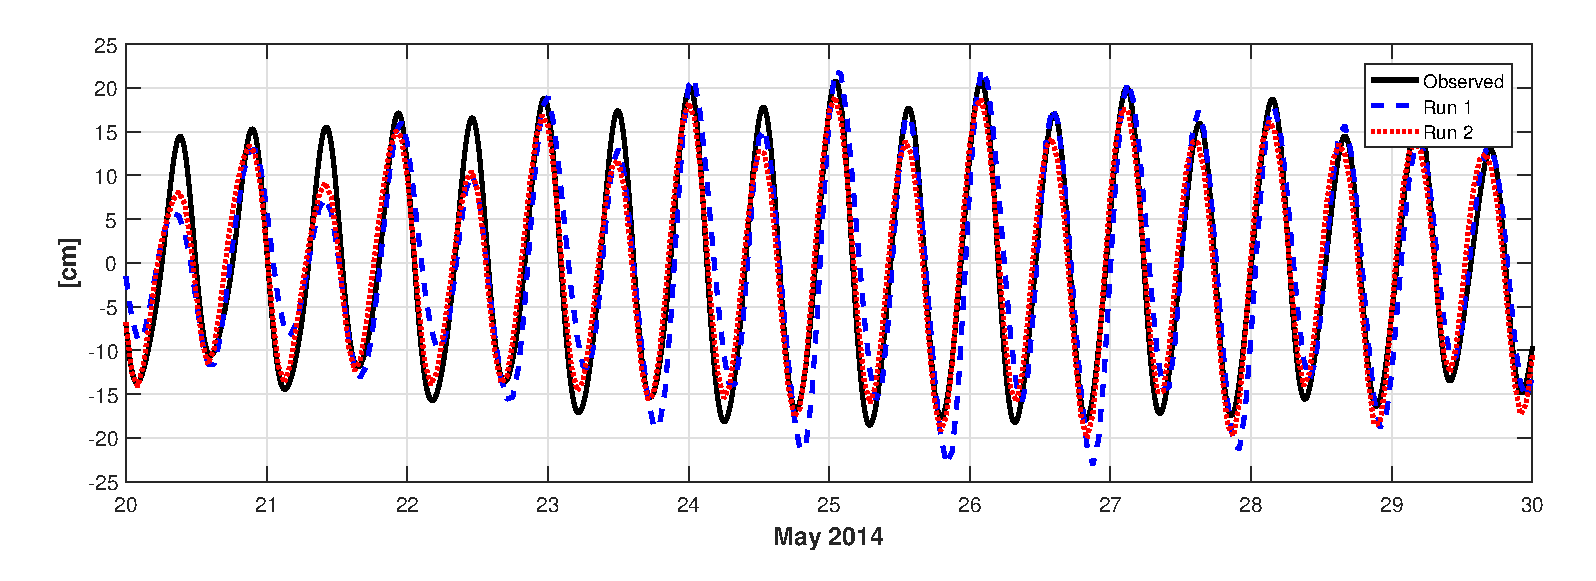
\includegraphics[width=\textwidth]{fig_Viker_timeseries}
\caption{Time series of water level at a position close to Viker in the Oslofjord}
\label{fig:Viker_timeseries}
\end{figure}



\begin{table}[ht]
%\vspace{-1.5cm}
\caption{Tidal amplitudes [cm] and phases [deg] for the water level at Viker in the Oslofjord together with adjustment factors $c^{(n)}$ and phase shifts $\triangle \phi^{(n)}$ for each component}
\label{tab:Viker}
\centering
\begin{tabular}{crrrrrrrrrr} \hline
       & Period & \multicolumn{2}{c}{Observed} & \multicolumn{2}{c}{Run 1} & \multicolumn{2}{c}{Run 2} & \multicolumn{2}{c}{Adjustment} \\
Comp.  & [h] $\;\;$ & [cm] & [deg] & [cm] & [deg] & [cm] & [deg] & $c^{(n)}$ & $\triangle \phi^{(n)}$  \\ \hline 
S$_2$  &  12.0000 &   3.0 &  39 &    5.1 &  81 &    3.2 &  67 &    0.588 &   -42.4   \\
M$_2$  &  12.4206 &  11.8 & 105 &    9.7 & 122 &   11.8 & 105 &    1.224 &   -16.8   \\
N$_2$  &  12.6584 &   3.4 &  57 &    5.7 &  81 &    3.1 &  69 &    0.595 &   -24.2   \\
K$_1$  &  23.9345 &   0.7 & 136 &    1.2 & 212 &    0.1 & 198 &    0.554 &   -75.9   \\
P$_1$  &  24.0659 &   0.5 &  66 &    1.2 & 212 &    0.1 & 198 &    0.424 &  -145.5   \\
O$_1$  &  25.8193 &   2.2 & 279 &    3.7 &  19 &    2.9 & 338 &    0.591 &   259.8   \\
MN$_4$ &   6.2692 &   0.4 & 263 &    1.0 & 141 &    0.3 &   7 &    0.368 &   122.2   \\
M$_4$  &   6.2103 &   1.2 & 275 &    0.7 &  25 &    1.1 & 354 &    1.742 &   249.2   \\
MS$_4$ &   6.1033 &   0.3 & 348 &    1.1 & 111 &    0.6 &  80 &    0.272 &   236.7   \\ \hline
\end{tabular}
\end{table}


\begin{table}[ht]
%\vspace{-1.5cm}
\caption{Tidal amplitudes [cm] and phases [deg] for the water level at Oscarsborg in the Oslofjord}
\label{tab:Oscarsborg}
\centering
\begin{tabular}{crrrrrrrrrr} \hline
      & Period & \multicolumn{2}{c}{Observed} & \multicolumn{2}{c}{Run 1} & \multicolumn{2}{c}{Run 2}  \\
Comp. & [h] $\;\;$ & [cm] & [deg] & [cm] & [deg] & [cm] & [deg]  \\ \hline 
S$_2$  & 12.0000 &  3.6 &  59  &   6.1 &  85  &  3.7 &  69.8  \\
M$_2$  & 12.4206 & 13.7 & 121  &  11.1 & 128  & 13.7 & 111.0  \\
N$_2$  & 12.6584 &  3.9 &  74  &   6.6 &  86  &  3.6 &  75.1  \\
K$_1$  & 23.9345 &  0.9 & 138  &   1.1 & 213  &  0.1 &  44.1  \\
P$_1$  & 24.0659 &  0.7 &  75  &   1.1 & 213  &  0.1 &  44.1  \\
O$_1$  & 25.8193 &  2.4 & 281  &   3.9 &  21  &  3.1 & 340.2  \\
MN$_4$ &  6.2692 &  0.6 & 308  &   2.0 & 163  &  0.5 &  29.1  \\
M$_4$  &  6.2103 &  1.7 & 319  &   1.4 &  44  &  2.0 &  14.5  \\
MS$_4$ &  6.1033 &  0.4 &  32  &   2.2 & 135  &  1.3 & 105.5  \\ \hline 
\end{tabular}
\end{table}




\begin{figure}[!t]
\centering
\includegraphics[trim=1cm 1cm 0cm 0cm,clip=true,width=0.49\textwidth]{fig_Oslofjorden_M2amp.eps}
\includegraphics[trim=1cm 1cm 0cm 0cm,clip=true,width=0.49\textwidth]{fig_Oslofjorden_M2phase.eps}
%\includegraphics[width=0.33\textwidth]{fig_Oslofjorden_M2camp.eps}
\caption{Fields of M$_2$ water level amplitude (left) and phase (right) in the Oslofjord. The corresponding observed values are indicated by coloured circles at the three permanent gauges in the area.}
\label{fig:Oslofjord_tidal_fields}
\end{figure}


\begin{figure}[!t]
\centering
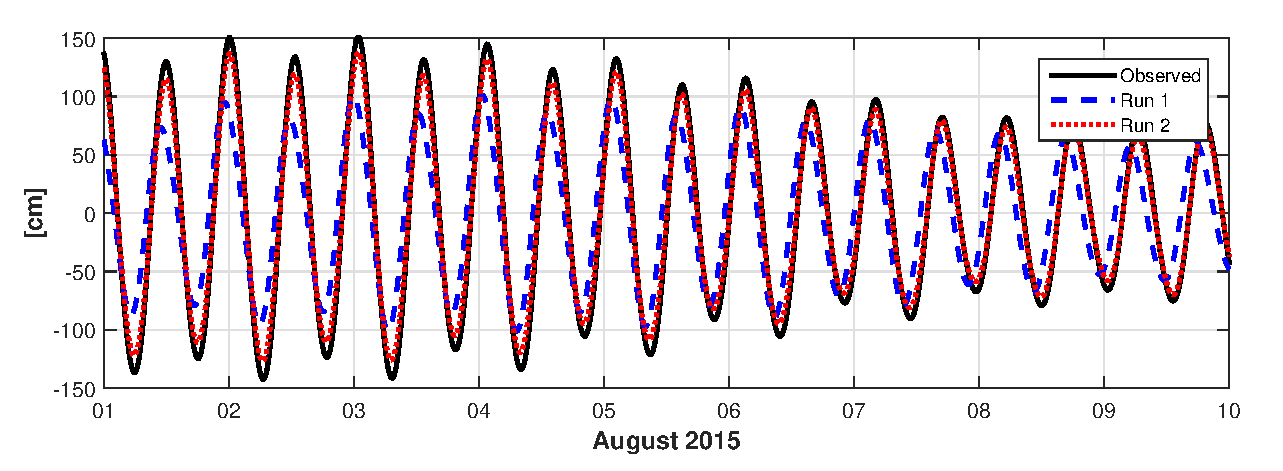
\includegraphics[width=\textwidth]{fig_Saltstraumen_timeseries}
\caption{Time series of water level at a position close to Bod{\o} in the Saltfjord}
\label{fig:Saltstraumen_timeseries}
\end{figure}


\begin{figure}[!t]
\centering
\includegraphics[width=\textwidth]{fig_Saltstraumen_M2amp}
\includegraphics[width=\textwidth]{fig_Saltstraumen_M2phase}
\caption{Fields of M$_2$ water level amplitude and phase in the Saltfjord model.}
\label{fig:Saltstraumen_field}
\end{figure}

\begin{table}[ht]
%\vspace{-1.5cm}
\caption{Tidal amplitudes [cm] and phases [deg] for the water level at Bod{\o} in the Saltfjord together with adjustment factors $c^{(n)}$ and phase shifts $\triangle \phi^{(n)}$ for each component}
\label{tab:Bodo}
\centering
\begin{tabular}{crrrrrrrrrr} \hline
      & Period & \multicolumn{2}{c}{Observed} & \multicolumn{2}{c}{Run 1} & \multicolumn{2}{c}{Run 2} & \multicolumn{2}{c}{Adjustment} \\
Comp. & [h] $\;\;$ & [cm] & [deg] & [cm] & [deg] & [cm] & [deg] & $c^{(n)}$ & $\triangle \phi^{(n)}$  \\ \hline 
S$_2$   & 12.0000  &  30.0 &      8   &  19.1 &     16   &  28.1 &      7    &   1.570  &    -7.2   \\ 
M$_2$   & 12.4206  &  87.3 &    331   &  60.0 &    301   &  78.3 &    330    &   1.454  &    29.8   \\ 
N$_2$   & 12.6584  &  18.5 &    308   &  12.7 &    271   &  16.7 &    309    &   1.461  &    37.2   \\ 
K$_1$   & 23.9345  &  10.8 &    194   &   8.8 &    183   &  10.7 &    194    &   1.225  &    11.5   \\ 
O$_1$   & 25.8193  &   3.8 &     33   &   3.3 &     39   &   3.7 &     33    &   1.154  &    -6.1   \\ 
MN$_4$  &  6.2692  &   1.5 &    229   &   0.4 &    122   &   1.5 &    228    &   3.000  &   106.9   \\ 
M$_4$   &  6.2103  &   2.7 &    268   &   3.3 &    159   &   3.1 &    283    &   0.808  &   109.5   \\ 
MS$_4$  &  6.1033  &   1.3 &      2   &   1.5 &    152   &   1.4 &     30    &   0.861  &  -149.6   \\ \hline
\end{tabular}
\end{table}

\begin{figure}[!t]
\centering
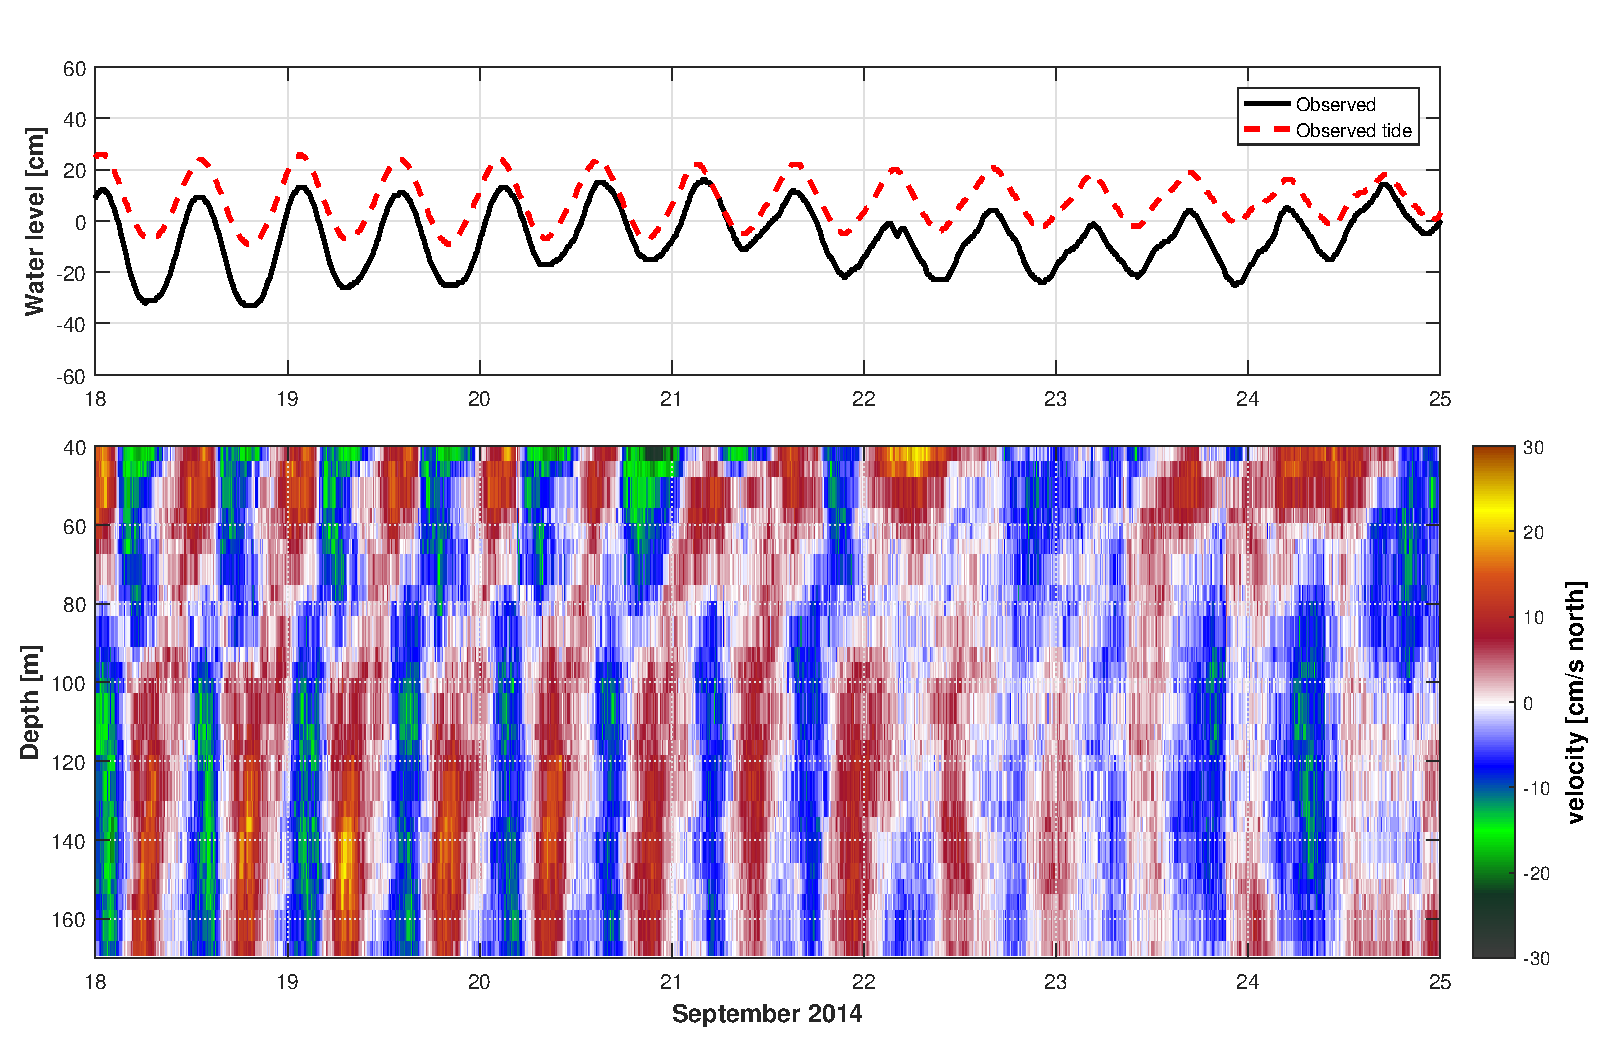
\includegraphics[width=\textwidth]{fig_Filtvedt_timeseries_obs}
\caption{Time series of water level at Oscarsborg (upper) and currents at a position close to Filtvedt (lower) in the Oslofjord. Observations at water depths less than 40 meters are not included due to noise in the upper levels.}
\label{fig:Filtvedt_timeseries_obs}
\end{figure}


\begin{figure}[!t]
\centering
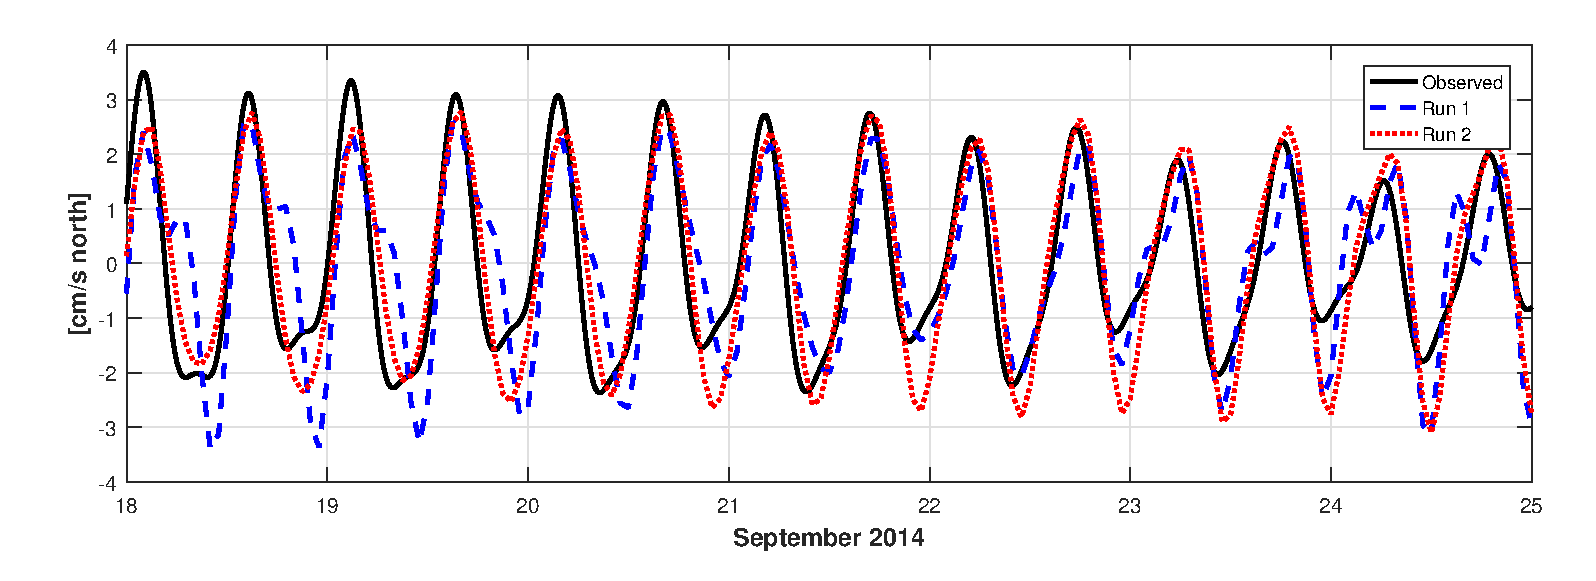
\includegraphics[width=\textwidth]{fig_Filtvedt_timeseries}
\caption{Time series of depth averaged tidal currents at a position close to Filtvedt in the Oslofjord. The time series are constructed based on the tidal components. Neither observed nor modelled currents at water depths less than 40 meters are included due to noise in the upper levels of the observations.}
\label{fig:Filtvedt_timeseries}
\end{figure}

%\begin{figure}[!t]
%\centering
%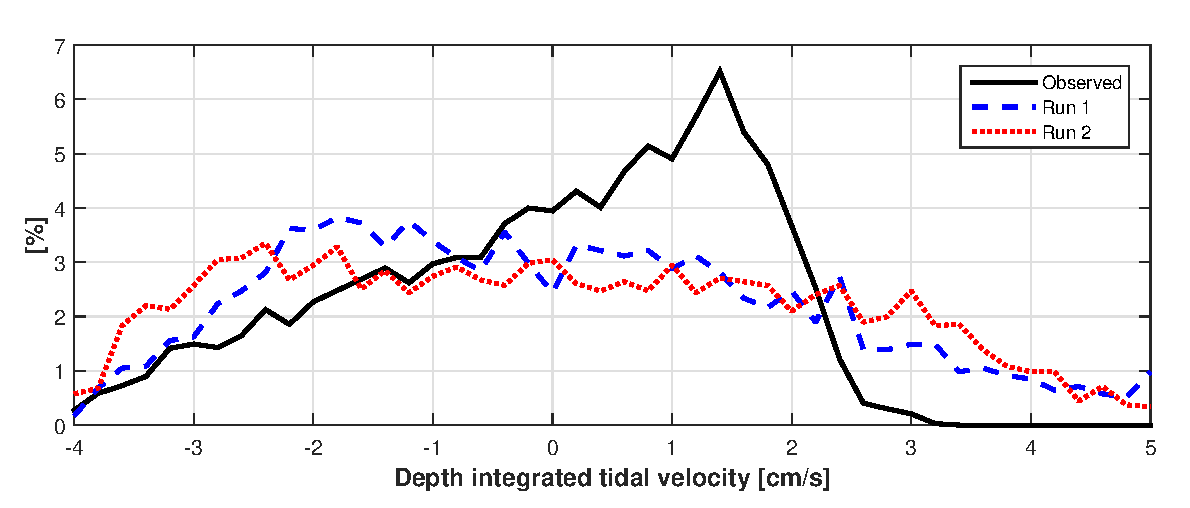
\includegraphics[width=\textwidth]{fig_Filtvedt_pdf}
%\caption{Probability density functions of observed and modelled depth integrated tidal currents at a position near Filtvedt in the Oslofjord. The bin width is here 0.1 cm/s. Only currents below 40 meters depth are included due to noise in the upper levels of the observations.}
%\label{fig:Filtvedt_pdf}
%\end{figure}


\begin{table}[ht]
%\vspace{-1.5cm}
\caption{Tidal major amplitudes [cm/s] and phases [deg] for the current near Filtvedt in the Oslofjord. The Root Mean Square Error (RMSE) for the time series of each component are computed.}
\label{tab:Filtvedt}
\centering
\begin{tabular}{crcrcrcrcc} \hline
      & Period & \multicolumn{2}{c}{Observed} & \multicolumn{2}{c}{Run 1} & \multicolumn{2}{c}{Run 2} & \multicolumn{2}{c}{RMSE} \\
Comp. & [h] $\;\;$ & [cm/s] & [deg] & [cm/s] & [deg] & [cm/s] & [deg] & Run 1 & Run 2\\ \hline 
S$_2$  & 12.0000 &  0.5 & 280  &   1.4 & 336  &  0.5 & 334  & 1.0 & 0.4 \\
M$_2$  & 12.4206 &  1.8 &   9  &   2.3 &  18  &  2.0 &  16  & 2.5 & 0.4 \\
N$_2$  & 12.6584 &  0.5 & 293  &   1.3 & 339  &  0.5 & 343  & 0.9 & 0.2 \\
K$_1$  & 23.9345 &  0.5 &  61  &   0.1 &   5  &  0.0 & 261  & 0.3 & 0.3 \\
%P$_1$  & 24.0659 &  -   &  -   &    -  &  -   &   -  &  -   \\
O$_1$  & 25.8193 &  0.1 & 120  &   0.3 & 244  &  0.2 & 250  & 0.2 & 0.1 \\
MN$_4$ &  6.2692 &  0.3 & 166  &   0.7 &  52  &  0.2 & 305  & 0.4 & 0.3 \\
M$_4$  &  6.2103 &  0.7 & 220  &   0.6 & 303  &  0.7 & 291  & 0.7 & 0.7 \\
MS$_4$ &  6.1033 &  0.0 & 252  &   0.8 &  24  &  0.4 &  19  & 0.6 & 0.2 \\
\hline 
\end{tabular}
\end{table}


\section{Conclusion}

A key factor to modelling currents in any ocean model is accurate tidal forcing. For regional models, this can be taken from a global or regional atlas of tides, like the TPXO or similar. Our experience is that these solutions might not produce adequate accurate results when applied at the mouth of a fjord in a fjord model. This is because the phase speed of the tidal wave can vary close to the coast, and that the coastline and the depth is not properly resolved in the coarse tidal atlases.

We have proposed a simple method to adjust tidal forcing. First we run the ocean model with tidal forcing based on the global or regional tidal atlas, for example the global TPXO with a resolution of $1/4$ degree. Secondly, we run harmonic analysis in order to compare the simulated and observed water level for each tidal component. The ratio between observed and simulated amplitude and a phase difference are computed for each tidal component, and then used to adjust the tidal forcing. The same ratio and phase difference is applied on the amplitudes of both water level and current. After this, the model is rerun with adjusted tidal forcing and the results are evaluated against observations.

The method is tested with the Regional Ocean Model System (ROMS) on two different fjords in Norway, the Oslofjord and the Saltfjord, which includes the famous Saltstraum maelstrom.
 
The results show improvements in the modelled tidal elevations and phases in both models, and suggest that this simple approach is one way of correcting coarse tidal atlases to yield improved results in a fjord model.


\bibliographystyle{apalike}
\bibliography{Bibliography_Tide}

\end{document}
